\section{Udvælgelse af skalaer}
\label{ParametreDatabehandlingSkalaer}
%


%NOGET OM HVORDAN PARAMETRENE ER "FUNDET" 
Ud fra de opstillede parametre, opstilles der skalaer, ved at gennemgå alle sætningerne markeret med S (for Scale). Kravet for opstilling af en skala er, at det er muligt at ændre på den specifikke parametre skalaen beskriver. Formålet er at opstille den optimale skala for hvert enkelt parameter, der er derfor ikke fastsat én specifik skala type på forhånd. 
%Det vurderes at en bipolær skala er mest beskrivende da den har den største spænd og denne vil derfor fortrækkes, i tilfælde hvor der findes både en bipolær og unipolær. 


%OBS: Nogen af de orange (Skalaer) er slået sammen, fordi de egentlig siger det samme og hører under det samme emne. 
% OBS: Jeg synes R er en god idé hører under grøn 8 (positiv overfor R) er sorteret fra fordi det ikke er noget der kan ændres på i forhold til robotten. 
%OBS: Det der handler om kendskab til teknologi beholdes som skalaer selvom det ikke er muligt at ændre på det. De vil blive brugt i forbindelse med indsamling af demografi, så det kan sammenholdes med resten af deres respons. (Jeg synes R minder om noget jeg kender er slået sammen med jeg har erfaring med robotter til Hvor meget kendskab har du til teknologi/robotter)

%OBS igang med at slå dem sammen efter hvad der hænger sammen (Dem der ikke nævnes her, står for sig selv)

%Anmassende, intimiderende og let at ignorer R bliver slået sammen - til: Jeg synes R er anmassende

%Jeg synes R ser menneskelig ud, Jeg synes R er levende og jeg foretrækker R ser menneskelig ud slåes sammen - Til: Jeg synes R er menneskelig

%Fjerner "Jeg kan godt lide R's udseende" fordi det formentlig er en overkategori til sej, sjov, sød, elegant, så hvis de rates højt er det formentlig et udtryk for at de også godt kan lide robottens udseende, hvorhvis sej, sjov, sød mm. rates dårligt er det et udtryk for at de ikke kan lide R's udseende. Så parameteren bliver målt indirekte, ved underparametre. 

%Jeg blev nysgerrige da jeg så R, jeg synes R er spændende og R fangede min opmærksomhed, bliver slået sammen til: Jeg synes R er spændende

%Jeg oplevede hastighed som værende langsom/hurtig og Jeg synes hastighed som værende langsom/hurtig slåes sammen til: Jeg synes Rs hastighed er for (langsom/hurtig) (slået sammen inden vi til sidst skal udvælge dem vi bruger)

%Jeg føler R kan hjælpe mig, R kan hjælpe mig så jeg ikke behøver at spørger personale, Jeg kan bruge R til at finde rundt i L slåes sammen til: Jeg føler at R kan hjælpe mig

%Jeg synes R's bevægelser er behagelige og Jeg synes R har rolige bevægelser er slået sammen til: Jeg synes R har (Rolige/vilde)

%Jeg oplevede R højdes som værende meget høj/lav og Jeg synes R's højde er for høj for lav bliver slået sammen til: Jeg synes R's højde er (høj/lav) (slået sammen inden vi til sidst skal udvælge dem vi bruger)



Når parametrene er udledt fra hver af de grønne kategorier skal der udvælges de parametre, som vil blive anvendt i forbindelse med at udvikle skalaerne. 

Fælles for disse parametre er, at de skal opfylde følgende kriterier: \blankline
%
\begin{itemize}
  \item En designer skal kunne ændre på det
  \item 
\end{itemize}



NOTER FRA DANNELSEN AF SKALAERNE:
\textbf{Jeg føler mig tryg ved R}
DEnne er baseret på observationer og ikke direkte udtalelser fra testpersonerne. 
Ekstrem tryg/

\textbf{Jeg regner med at R følger mig hen til det sted jeg har valgt} 
helt enig/helt uenig med neutral i midten. 

Vilde bevægelser vælges som modpol til rolige bevægelser da det vurderes at være modsætningen, men også i høj grad fordi denne beskrivelse blev brugt af testpersonerne i undersøgelsen. 

Blev sorteret fra da den ikke er manipulerbar, da den kun henvender sig til hvad man foretrækker. \blankline


%
\begin{figure}[H]
\centering
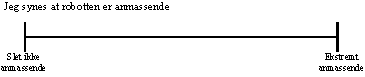
\includegraphics[width =\textwidth]{Figure/UdvalgteSkalaer/Anmassende} 
\caption{NY.}
\label{fig:SkalaAnmassende}
\end{figure}
\noindent
%

%
\begin{figure}[H]
\centering
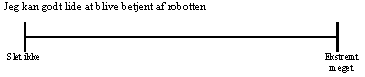
\includegraphics[width =\textwidth]{Figure/UdvalgteSkalaer/BetjeningAfR} 
\caption{NY.}
\label{fig:SkalaBetjeningAfR}
\end{figure}
\noindent
%

%
\begin{figure}[H]
\centering
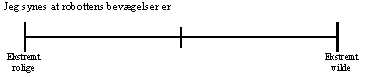
\includegraphics[width =\textwidth]{Figure/UdvalgteSkalaer/BevaegelserR} 
\caption{NY.}
\label{fig:SkalaBevaegelserR}
\end{figure}
\noindent
%

%
\begin{figure}[H]
\centering
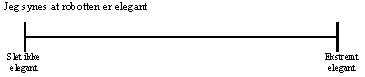
\includegraphics[width =\textwidth]{Figure/UdvalgteSkalaer/ElegantR} 
\caption{NY.}
\label{fig:SkalaElegantR}
\end{figure}
\noindent
%

%
\begin{figure}[H]
\centering
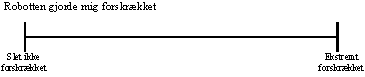
\includegraphics[width =\textwidth]{Figure/UdvalgteSkalaer/Forskraekket} 
\caption{NY.}
\label{fig:SkalaForskraekket}
\end{figure}
\noindent
%

%
\begin{figure}[H]
\centering
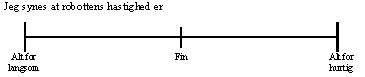
\includegraphics[width =\textwidth]{Figure/UdvalgteSkalaer/HastighedR} 
\caption{NY.}
\label{fig:SkalaHastighedR}
\end{figure}
\noindent
%

%
\begin{figure}[H]
\centering
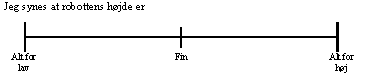
\includegraphics[width =\textwidth]{Figure/UdvalgteSkalaer/HoejdeR} 
\caption{NY.}
\label{fig:SkalaHoejdeR}
\end{figure}
\noindent
%

%
\begin{figure}[H]
\centering
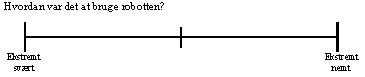
\includegraphics[width =\textwidth]{Figure/UdvalgteSkalaer/HvordanVarDetAtBrugeR} 
\caption{NY.}
\label{fig:SkalaHvordanVarDetAtBrugeR}
\end{figure}
\noindent
%

%
\begin{figure}[H]
\centering
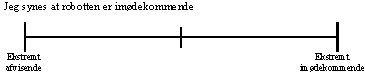
\includegraphics[width =\textwidth]{Figure/UdvalgteSkalaer/Imoedekommende} 
\caption{NY.}
\label{fig:SkalaImoedekommende}
\end{figure}
\noindent
%

%
\begin{figure}[H]
\centering
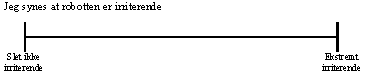
\includegraphics[width =\textwidth]{Figure/UdvalgteSkalaer/Irriterende} 
\caption{NY.}
\label{fig:SkalaIrriterende}
\end{figure}
\noindent
%

%
\begin{figure}[H]
\centering
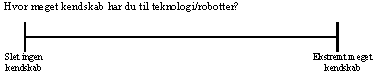
\includegraphics[width =\textwidth]{Figure/UdvalgteSkalaer/KendskabTilTeknologi} 
\caption{NY.}
\label{fig:SkalaKendskabTilTeknologi}
\end{figure}
\noindent
%

%
\begin{figure}[H]
\centering
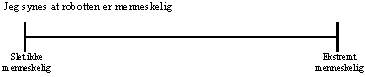
\includegraphics[width =\textwidth]{Figure/UdvalgteSkalaer/MenneskeligR} 
\caption{NY.}
\label{fig:SkalaMenneskeligR}
\end{figure}
\noindent
%

%
\begin{figure}[H]
\centering
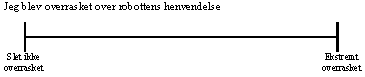
\includegraphics[width =\textwidth]{Figure/UdvalgteSkalaer/OverrasketOverR} 
\caption{NY.}
\label{fig:SkalaOverrasketOverR}
\end{figure}
\noindent
%

%
\begin{figure}[H]
\centering
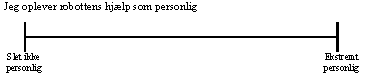
\includegraphics[width =\textwidth]{Figure/UdvalgteSkalaer/PersonligHjaelp} 
\caption{NY.}
\label{fig:SkalaPersonligHjaelp}
\end{figure}
\noindent
%

%
\begin{figure}[H]
\centering
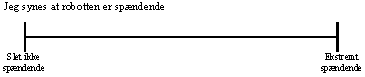
\includegraphics[width =\textwidth]{Figure/UdvalgteSkalaer/RerSpaendende} 
\caption{NY.}
\label{fig:SkalaRerSpaendende}
\end{figure}
\noindent
%

%
\begin{figure}[H]
\centering
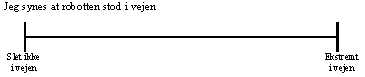
\includegraphics[width =\textwidth]{Figure/UdvalgteSkalaer/RobottenErIVejen} 
\caption{NY.}
\label{fig:SkalaRerIVejen}
\end{figure}
\noindent
%

%
\begin{figure}[H]
\centering
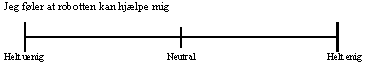
\includegraphics[width =\textwidth]{Figure/UdvalgteSkalaer/RobottenKanHjaelpe} 
\caption{NY.}
\label{fig:SkalaRKanHjaelpe}
\end{figure}
\noindent
%

%
\begin{figure}[H]
\centering
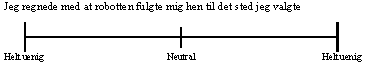
\includegraphics[width =\textwidth]{Figure/UdvalgteSkalaer/RobottenFulgteMigDetRigtigeStedHen} 
\caption{NY.}
\label{fig:SkalaRFulgteMigDetRigtigeStedHen}
\end{figure}
\noindent
%

%
\begin{figure}[H]
\centering
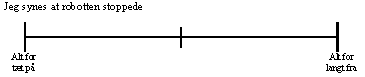
\includegraphics[width =\textwidth]{Figure/UdvalgteSkalaer/RStoppede} 
\caption{NY.}
\label{fig:SkalaRStoppede}
\end{figure}
\noindent
%

%
\begin{figure}[H]
\centering
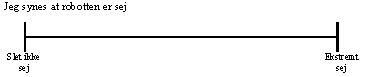
\includegraphics[width =\textwidth]{Figure/UdvalgteSkalaer/SejR} 
\caption{NY.}
\label{fig:SkalaSejR}
\end{figure}
\noindent
%

%
\begin{figure}[H]
\centering
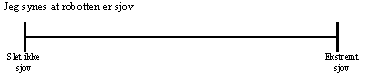
\includegraphics[width =\textwidth]{Figure/UdvalgteSkalaer/SjovR} 
\caption{NY.}
\label{fig:SkalaSjovR}
\end{figure}
\noindent
%

%
\begin{figure}[H]
\centering
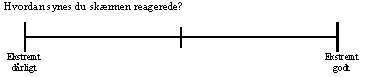
\includegraphics[width =\textwidth]{Figure/UdvalgteSkalaer/SkaermensReaktion} 
\caption{NY.}
\label{fig:SkalaSkaermensReaktion}
\end{figure}
\noindent
%

%
\begin{figure}[H]
\centering
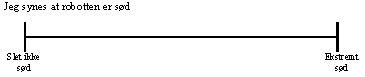
\includegraphics[width =\textwidth]{Figure/UdvalgteSkalaer/SoedR} 
\caption{NY.}
\label{fig:SkalaSoedR}
\end{figure}
\noindent
%

%
\begin{figure}[H]
\centering
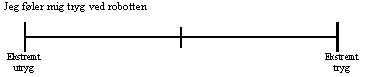
\includegraphics[width =\textwidth]{Figure/UdvalgteSkalaer/TrygVedR} 
\caption{NY.}
\label{fig:SkalaTrygVedR}
\end{figure}
\noindent
%
